\section{Limitations in how we've been optimizing so far}

\begin{frame}

Our iterative gradient-based optimizations:
\begin{itemize}
\item assumes the optimum ``up ahead'' is the best solution,

\begin{figure}[ht]
  \centering
  \begin{tabular}{c c}
      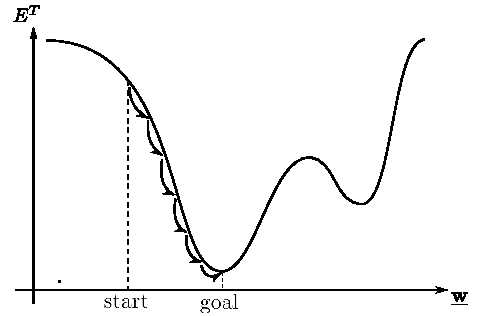
\includegraphics[height=3.5cm]{img/gradient-descent.pdf} &
      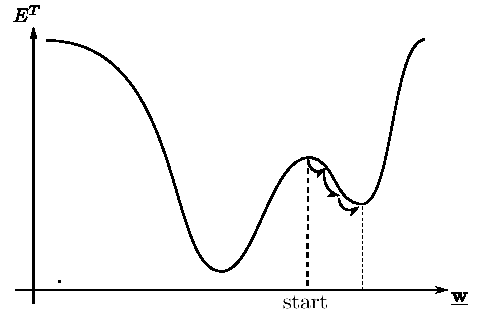
\includegraphics[height=3.5cm]{img/gradient-descent_local.pdf}
  \end{tabular}
  \notesonly{
  \caption{Learning by gradient descent}\label{fig:graddescent}
  }
\end{figure}

\item doesn't handle discrete optimization.
\end{itemize}

\end{frame}
